\documentclass[jou]{apa6}
%\documentclass[11pt]{article}
\usepackage{ucs}
\usepackage[utf8x]{inputenc}
\usepackage{changepage}
\usepackage{graphicx}
\usepackage{amsmath}
\usepackage{gensymb}
\usepackage{amssymb}
\usepackage{enumerate}
\usepackage{tabularx}
\usepackage{lipsum}
\usepackage{hyperref}
\usepackage[framemethod=TikZ]{mdframed}

\oddsidemargin 0.0in
\evensidemargin 0.0in
\textwidth 6.27in
\headheight 1.0in
\topmargin -0.1in
\headheight 0.0in
\headsep 0.0in
\textheight 9.0in

\usepackage{xcolor}

\setlength\parindent{0pt}

\newenvironment{myenv}{\begin{adjustwidth}{0.4in}{0.4in}}{\end{adjustwidth}}
\renewcommand{\abstractname}{Anotācija}
\renewcommand\refname{Atsauces}



\newcounter{alphnum}
\newenvironment{alphlist}{\begin{list}{(\Alph{alphnum})}{\usecounter{alphnum}\setlength{\leftmargin}{2.5em}} \rm}{\end{list}}


%16.3-6

\makeatletter
\let\saved@bibitem\@bibitem
\makeatother

\usepackage{bibentry}

\title{Homework 4}
\author{Discrete Structures}
\affiliation{RBS}

\begin{document}

\thispagestyle{empty}

\twocolumn
{\Large Discrete Homework 4}


\vspace{4pt}
{\bf Problem 1 (Rosen2019, \#60, p.649)} \textendash{} {\em After 9.5.}\\
{\bf (A)} Let $R$ be the relation on the set of functions from $\mathbb{Z}^{+}$ to 
$\mathbb{Z}^{+}$ such that $(f,g)$ belongs to $R$ if and only if $f$ is
$\Theta(g)$ (see Section 3.2). Show that $R$ is an equivalence relation.\\
{\bf (B)} Describe the equivalence class containing $f(n) = n^2$ for this 
equivalence relation. (Your description could 
use predicate/quantifier expression satisfied by 
all functions $h\,:\,\mathbb{Z}^{+} \rightarrow \mathbb{Z}^{+}$ 
equivalent to $f(n) = n^2$.)

{\em Note.} Big-Theta Definition (Rosen2019): Function $f(x)$
is in $\Theta(g)$ iff there are positive real numbers $C_1$ and $C_2$ and a positive 
real number $k$ such that 
$$C_1\left| g(x) \right| \leq \left| f(x) \right| \leq C_2 \left| g(x) \right|$$
whenever $x > k$. (See Definition 3 on p.227.)\\
%{\em Note 2.} The usual Big-O notation is not an equivalence relation, because
%it is not symmetric. For example, function $f(n) = n$ is in $O(g(n))$, where
%$g(n) = n^2$. But $g(n)$ is not in $O(f(n))$. Namely, linear function $f(n) = n$ 
%is bounded from above by a quadratic function $g(n) = n^2$, but not vice versa.

\vspace{6pt}
{\bf Problem 2 (Rosen2019, \#64, p.649)} \textendash{} {\em After 9.5.}\\
Do we necessarily get an equivalence relation when we form the symmetric closure of 
the reflexive closure of the transitive closure of a relation?

{\em Note.} Terms {\em reflexive closure} and {\em symmetric closure} are defined in 
(Rosen2019, p.628). The reflexive closure of a binary relation $R$ is 
the smallest relation containing $R$ that is reflexive: 
$R_1$ is obtained from $R$ by adding to it all pairs $(a,a)$ (unless they 
are already in $R$). The {\em symmetric closure} of a binary 
relation $R$ is the smallest relation $R_2$ containing $R$ that is symmetric 
(if pair $(a,b)$ belongs to $R$, then both 
pairs $(a,b)$ and $(b,a)$ are added to $R_2$). 

\vspace{6pt}
{\bf Problem 3.}\\
Suppose that winners of some lottery make a set $X$. 
Each winner should receive two prizes from some prize collection $Y$.
For each subset of the set of winners $S \subseteq X$ the set 
of prizes $N(S) \subseteq Y$ wanted by one or more people $p \in S$ satisfy 
$$|N(S)| \geq 2|S|.$$
Show that every winner can be given two prizes that s/he wants.
({\em Inspired by (Rosen2019, \#33, p.701)}.)
%% https://www.epfl.ch/labs/dcg/wp-content/uploads/2018/10/GT-ProblemSet3-Solutions.pdf


\vspace{6pt}
{\bf Problem 4 (Rosen2019, \#66, p.728)} \textendash{} {\em After 10.4.}\\
Suppose that you have a three-gallon jug and a five-gallon jug. 
You may fill either jug with water, you may empty either 
jug, and you may transfer water from either jug into the other jug [until it is full].\\ 
{\bf (A)} Use a path in a directed graph to show that you can end up with a jug containing
exactly one gallon.\\
{\bf (B)} How many vertices and how many edges are there in this directed graph?\\
(In order to build this graph of available states
use an ordered pair $(a,b)$ to indicate how much water is in each jug. Represent these ordered
pairs by vertices. Add an edge for each operation with the jugs.)

\vspace{6pt}
{\bf Problem 5 (Rosen2019, \#22, p.792)} \textendash{} {\em After 11.1.}\\
A chain letter starts when a person sends a letter to five others. 
Each person who receives the letter either sends it to five other people
who have never received it or does not send it to anyone. Suppose that 
$10,000$ people send out the letter before the chain ends and that no one receives
more than one letter. How many people receive the letter, and how many 
do not send it out?


\vspace{6pt}
{\bf Problem 6 (Rosen2019, \#46, p.793)} \textendash{} {\em After 11.1.}\\
How many vertices, leaves, and internal vertices does the rooted Fibonacci tree
$F_n$ have, where $n$ is a positive integer? What is its height?

{\em Note} The {\em rooted Fibonacci trees} $T_n$ are defined recursively 
in the following way. $T_1$ and $T_2$ are both the rooted tree consisting
of a single vertex, and for $n=3,4,\ldots$, the rooted tree $T_n$ 
is constructed from a root with $T_{n-1}$ as its left subtree and $T_{n-2}$
as its right subtree.



\vspace{6pt}
{\bf Problem 7 (Rosen2019, \#25, p.820)} \textendash{} {\em After 11.3.}\\
Construct the ordered rooted tree whose preorder traversal is 
$a,b,f,c,g,h,i,d,e,j,k,l$, where $a$ has four children, $c$ has three children, 
$j$ has two children, $b$ and $e$ have one child each, and all other vertices are leaves.

\vspace{6pt}
{\bf Problem 8.}
Assume that somebody wants to solve the following olympiad problem using ``brute force'':
\begin{mdframed}[roundcorner=6pt]
{\em Insert any arithmetic operation symbols ($+$, $-$, $\cdot$ and $/$) and
parentheses to get a correct equality:}\\
{\bf (A)} $3\;\;\;3\;\;\;7\;\;\;7\,=\,14$,\\
{\bf (B)} $3\;\;\;3\;\;\;7\;\;\;7\,=\,24$.\\
({\em \url{https://bit.ly/2JsXH5P}; Pg.1, P3.})
\end{mdframed}
How many different rooted trees can be obtained?
In Grade 5 there is no ``unary minus'' such as $(-3)\cdot 3$;
all four arithmetic operations are binary.

{\em Note.} 
You do not need to solve the quoted olympiad 
problem itself. Just count the possible expressions on the left side
that differ either by the syntax tree or by operation(s).

\vspace{6pt}
{\bf Problem 9 (Rosen2019, \#56, p.834)} \textendash{} {\em After 11.4.}\\
Show that it is possible to find a sequence of spanning trees leading from any spanning tree
to any other by successively removing one edge and adding another.

\vspace{6pt}
{\bf Problem 10 (Rosen2019, \#33, p.840)} \textendash{} {\em After 11.5.}\\
Show that if $G$ is a weighted graph with distinct edge weights, then for every simple
circuit of $G$, the edge of maximum wieght in this circuit 
does not belong to any minimum spanning tree of $G$.



\newpage

\section{Answers}


{\bf Problem 4}\\
Every manipulation with water jugs reaches a final 
state where either some jug is empty or some jug is full 
(or both). Each pair of two water quantities $(w_x,w_y)$
can be represented by a point in the Cartesian coordinates. 
Filling or emptying the 5-gallon jug means moving left or right 
on a horizontal line ($x$ coordinate changes, but $y$ stays the same). 
Filling or emptying the 3-gallon jug means moving up or down 
on a vertical line ($y$ coordinate changes, but $x$ stays the same). 
It is also possible to transfer water from one jug to another 
until we reach a limit \textendash{} this means moving a 
point on a line with slope $-1$. 

{\bf (A)} Measuring 1 gallon is shown in Figure~\ref{fig:water-jugs-path}. 
Verbally it can be described as a sequence of $4$ steps:
\begin{itemize}
\item Initially both jugs are empty; fill the $3$ gallon jug. 
(Move from $(0;0)$ to $(0;3)$.)
\item Transfer all water from it into the $5$-gallon jug. 
(Move from $(0;3)$ to $(3;0)$.)
\item Fill the $3$-gallon jug again. (Move from $(3;0)$ to $(3;3)$.)
\item Transfer water into the $5$-gallon jug until it is full. 
At that point the $3$-gallon jug contains $1$ gallon of water.
(Move from $(3;3)$ to $(5;1)$.)
\end{itemize}

This sequence of steps is possible because of the 
Bezout identity for two mutual primes
$3$ and $5$: 
$$1 = 2\cdot 3 + (-1) \cdot 5.$$
Similar construction to get $1$ gallon is possible for any 
other jug volumes that are mutual primes.



\begin{figure}[!htb]
\center{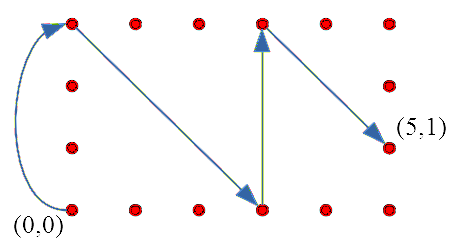
\includegraphics[width=2in]{hw04/water-jugs-path.png}}
\caption{\label{fig:water-jugs-path} Jugs: Measuring 1 gallon.}
\end{figure}


{\bf (B)} Figure~\ref{fig:water-jugs} shows the complete graph of all 
states. Some of the edges are unidirectional, and some of them are
bidirectional (water can be transfered in either direction).
There are $6$ bidirectional vertical arrows (of length $3$) 
and $4$ bidirectional 
horizontal arrows (of length $5$) \textendash{} they move from one side of the
rectangle to another side. There are $7$ slanted bidirectional arrows. 
And there are also $12$ points on the sides of the rectangle (except the
corners). Each one can move to corners on either side of it \textendash{}
so there are $24$ unidirectional arrows. The total number of arrows is
$$2 \cdot (10 + 7) + 24 = 58.$$

{\em Answer.} The total number of vertices in this graph is $16$; the total number of
directed edges is $58$. And just $4$ edges are used to measure $1$ gallon
in Figure~\ref{fig:water-jugs-path}.




\begin{figure}[!htb]
\center{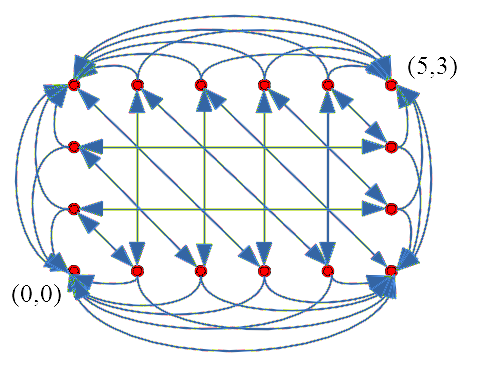
\includegraphics[width=2in]{hw04/water-jugs.png}}
\caption{\label{fig:water-jugs} Jugs: Graph of States.}
\end{figure}





\vspace{10pt}
{\bf Problem 5}\\
Since we know that exactly $10000$ people send out 
five letters each (and no one gets more than one letter), 
there are altogether $50000$ recipients. 

The number of people who do not send it out equals to the number 
of leaves in this tree. Moreover, there must be 
exactly $10000-1 = 9999$ inner nodes that are not the root. 
They got a letter, and also sent it out themselves. 
The remaining $50000 - 9999 = 40001$ recipients got the letter, 
but did not send it out.

{\em Answer.} $50000$ and $40001$.


A chain letter starts when a person sends a letter to five others. 
Each person who receives the letter either sends it to five other people
who have never received it or does not send it to anyone. Suppose that 
$10,000$ people send out the letter before the chain ends and that no one receives
more than one letter. How many people receive the letter, and how many 
do not send it out?


\vspace{6pt}
{\bf Problem 6}\\
Figure~\ref{fig:fibonacci-trees} shows the first six Fibonacci trees. 

\begin{figure}[!htb]
\center{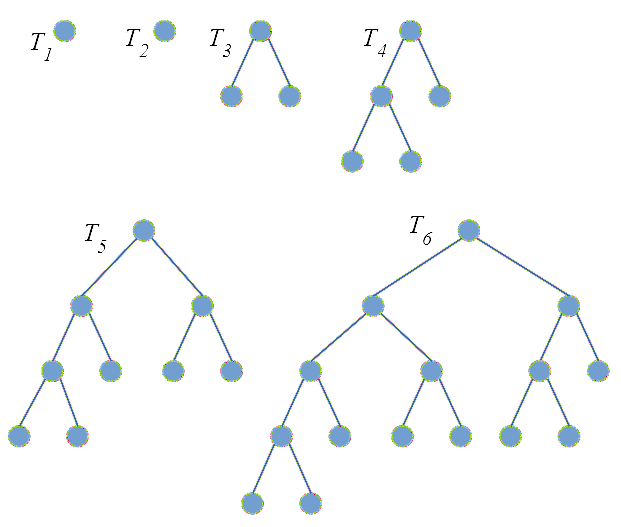
\includegraphics[width=2in]{hw04/fibonacci-trees.png}}
\caption{\label{fig:fibonacci-trees} Fibonacci trees.}
\end{figure}

We count the necessary elements in these trees (see table).

\begin{tabular}{|l|l|l|l|l|} \hline
Tree & Vertices & Leaves & Internal & Height \\ \hline
$T_1$ & $1$ & $1$ & $0$ & $0$ \\ \hline
$T_2$ & $1$ & $1$ & $0$ & $0$ \\ \hline
$T_3$ & $3$ & $2$ & $1$ & $1$ \\ \hline
$T_4$ & $5$ & $3$ & $2$ & $2$ \\ \hline
$T_5$ & $9$ & $5$ & $4$ & $3$ \\ \hline
$T_6$ & $15$ & $8$ & $7$ & $4$ \\ \hline
\end{tabular}

The easiest pattern is for the height. At every stage it grows by $1$, and for all $n > 2$: 
\begin{equation}
H(T_n) = n-2.
\end{equation}
The number of leaves in such trees satisfies the same recursive law
as the Fibonacci numbers: $L(T_{n}) = L(T_{n-1}) + L(T_{n-2})$. 
Also the first two values $L(T_1)$ and $L(T_2)$ are equal to the respective
Fibonacci numbers: $F(1) = F(2) = 1$. For this reason: 
\begin{equation}
L(T_n) = F(n).
\end{equation}

In any full binary tree the number of internal nodes is one less
than the number of leaves.
(Remember that a binary tree is called {\em full}, if any vertex is either a leaf or 
it has exactly two children.) We get 
\begin{equation}
I(T_n) = F(n) -1.
\end{equation}

The total number of vertices is the total of leaves and internal nodes. 
\begin{equation}
V(T_n) = 2F(n)-1.
\end{equation}











\vspace{6pt}
{\bf Problem 7}

As we construct the tree, we use data structure called ``stack''
(last-in-first-out). 
At the very beginning push the root on the stack \textendash{} 
this is the first vertex in the preorder; vertex $a$ with $4$ prospective children.
Every time there is a new vertex, we perform the following steps: 
\begin{enumerate}[(1)]
\item Pop off (i.e. delete from the stack) all those vertices, which
have all there ``child vacancies'' filled. 
\item Decrease by $1$ the child counter for the first non-nonzero vertex currently on the stack. 
\item Push (i.e. append as the last element on the stack) a new vertex with its child counter. 
BTW, this newly pushed vertex 
\item When all the child counters drop to $0$ the stack becomes empty and the algorithm stops.
\end{enumerate}

Every line below represents state of the stack at every given moment.

\begin{verbatim}
a(4)
a(3) b(1) 
a(3) b(0) f(0)
a(2) c(3)
a(2) c(2) g(0)
a(2) c(1) h(0)
a(2) c(0) i(0)
a(1) d(0)
a(0) e(1)
a(0) e(0) j(2) 
a(0) e(0) j(1) k(0)
a(0) e(0) j(0) l(0)
\end{verbatim}

When we draw the vertices in a rooted ordered graph, it looks like 
Figure~\ref{fig:tree0}.

\begin{figure}[!htb]
\center{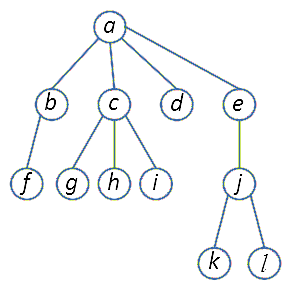
\includegraphics[width=1.5in]{hw04/tree0.png}}
\caption{\label{fig:tree0} Two spanning trees.}
\end{figure}



{\bf Problem 8}\\
Altogether there are $5$ ordered rooted trees with exactly $4$ leaves (and $3$ inner nodes). 
They correspond to the following parenthesized expressions (arithmetic operations are not shown):
$$((a\circ{}b)c)d\;\;(a(b\circ{}c))d\;\;(a\circ{}b)(c\circ{}d)\;\;a((b\circ{}c)d)\;\;a(b(cd)).$$

The five corresponding syntax trees are shown in Figure~\ref{fig:syntaxtree}. 

\begin{figure}[!htb]
\center{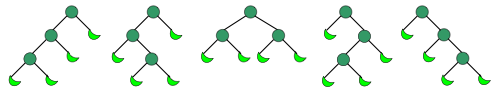
\includegraphics[width=3in]{hw04/syntaxtree.png}}
\caption{\label{fig:syntaxtree} Five syntax trees.}
\end{figure}

All the inner nodes in all these $5$ trees are distinguishable: just one of the inner nodes
is the root (the last operation in the tree); and for all the other inner nodes we know, 
in which subtree (or a subtree of a subtree) it is located. 
Since there are just $4$ arithmetic operations, there are $5 \cdot 4^3 = 320$: 
We get in total $320$ different ways how to restore parentheses and arithmetic operations in 
this example. So, the ``brute force'' is certainly possible for this problem, 
but it would not be easy for the 12 year olds (students in Grade 5), 
and one can easily miss something.





\vspace{10pt}
{\bf Problem 9}\\
Consider two spanning trees $T_1$ and $T_2$ on the same graph $G=(V,E)$. 
This means that both $T_1$ and $T_2$ contain all vertices of $G$, and they 
are both connected acyclic graphs (their edges are sufficient to create a path from any vertex
to any other in exactly one way).

Initially, the edges of $T_1$ and $T_2$ may be exactly the same (in this case we are done). 
Their edges may partially overlap. Or they may be completely disjoint (see the red/continuous 
and the blue/dashed spanning trees in the graph shown in Figure~\ref{fig:tree1}. 

\begin{figure}[!htb]
\center{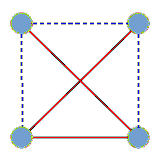
\includegraphics[width=0.6in]{hw04/tree1.png}}
\caption{\label{fig:tree1} Two spanning trees.}
\end{figure}

Assume that there is an edge $e=(v_i,v_j)$ in $T_1$ not included in $T_2$ (and there 
should also be an edge in $T_2$ not included in $T_1$, since both of them have the same
number of edges: $|V|-1$; one less than the number of vertices). 

If we drop the edge $e$ from $T_1$, then the vertices of $T_1$ falls apart into 
two disjoint pieces (one of them may consist of one vertex). Namely, 
$V = V' \cup V''$, where $V'$ and $V''$ are disjoint; and in $T_1$ there are no 
remaining edges (except $e=(v_i,v_j)$) connecting the sets $V'$ and $V''$. 

Consider the edges from $T_2$. There should be at least one edge going from one 
disconnected piece $V'$ to another piece $V''$. 
Take any edge from $T_2$ and add it to the edges of $T_1$ (to replace the recently removed edge $e$). 
After this step the overlap of edges in $T_1$ and $T_2$ increases by $1$. 
If we repeat such steps in a similar manner, eventually $T_1$ and $T_2$ will coincide.

\vspace{10pt}
{\bf Problem 10}\\
Proof by contradiction. We formulate the negation of what we have to prove. 
\begin{itemize}
\item Assume that there is some minimum spanning tree (MST) $T$ built on 
the edges of graph $G$
\item Assume that the graph $G$ has edge weights that are pairwise different
\item Assume thereis a simple circuit (i.e. circuit that does not use any edge twice) in $G$; 
and that circuit contains an edge $e = (v_i,v_j)$ that has the maximum weight in this circuit. 
\item Assume that the MST $T$ contains this edge $e$.
\end{itemize}

We will show that $T$ cannot, in fact be the minimum spanning tree; it is possible to 
find another spanning tree having even smaller total weight. 
Indeed, we can cut the edge $e = (v_i,v_j)$. Since $T$ is a tree, it falls apart into 
two pieces $T_1$ and $T_2$ such that $v_i$ is in $T_1$, $v_j$ is in $T_2$; both trees
$T_1$ and $T_2$ are not connected. 

Inspect the vertices that belong to the circuit $C$ consisting from the edges of the graph $G$. 
Color vertices belonging to $T_1$ white, and vertices belonging to $T_2$ black. 
We just saw that $(v_i,v_j)$ is an edge that goes from a white vertex to a black one. 
But there should be another edge $e'=(v_m,v_n)$ going back from black to white, since 
$C$ is a circuit that eventually loops back to the original vertex $v_i$. 

We can now connect pieces $T_1$ and $T_2$ using that new edge $e'$ (if there are many such edges, 
pick any one). We have created a new spanning tree $T'$ that is obtained by removing edge
$e=(v_i,v_j)$ and adding back another edge $e'=(v_m,v_n)$.
We claim that the weight $w(e') < w(e)$ (all edge weights are different; and $w(e)$ is the 
largest weight in that circuit). Therefore the new spanning tree $T'$ has smaller total weight than $T$. 
And $T$ cannot be the minimum spanning tree. It is a contradiction.


\end{document}



